\section{Introduzione}
\subsection{Contesto Applicativo}
\begin{frame}{Convenzione}
Una Convenzione è un accordo fra l'Università, rappresentata da un docente, ed una azienda per la realizzazione di un prodotto.

Una convenzione attraversa le seguenti fasi :\\
\vskip3ex
  \begin{enumerate}
    \item Il docente si accorda con un'azienda riguardo ad un progetto.
    \item Il docente, insieme al RAS, valuta i costi e stila la Tabella di Ripartizione dei compensi.
    \item Il RAS prepara un documento da discutere nel prossimo Consiglio di Dipartimento, che deciderà se approvare o meno la convenzione.
    \item In caso di approvazione la convenzione viene \textbf{inserita nell'applicazione}.
    \item ...
    \item La convenzione risulta esaurita (l'importo stabilito è stato pagato interamente) .
  \end{enumerate}
\end{frame}

\begin{frame}{Gestione di una Convenzione}
 L'applicazione deve monitorare la convenzione dal suo inserimento fino a quando risulti esaurita. 
 \vskip3ex
 In questo intervallo di tempo l'applicazione deve consentire di compiere delle operazioni sulla convenzione
\end{frame}

\subsection{Requisiti}
\begin{frame}{Requisiti principali}
  L'applicazione deve consentire di:\\
  \begin{itemize}
   \item inserire convenzioni
   \item inserire rate per una convenzione
   \item visualizzare le convenzioni inserite
   \item notificare le scadenze
  \end{itemize}

\end{frame}

\section{Analisi}
  \begin{frame}{Agenti}
    
    \begin{itemize}
     \item L'Operatore:\\
      \begin{itemize}
       \item inserisce, modifica convenzioni
       \item inserisce le rate
      \end{itemize}

     \item Il Docente:\\
      \begin{itemize}
       \item visualizza lo stato delle proprie convenzioni
      \end{itemize}

     \item Il Tempo:\\
      \begin{itemize}
       \item notifica le scadenze
      \end{itemize}

    \end{itemize}

    
  \end{frame}

  \subsection{Casi d'Uso}
  \begin{frame}{Casi d'uso dell'Operatore}
    \begin{figure}[h]
    \label{use_case_diag_operator}
    \centering
    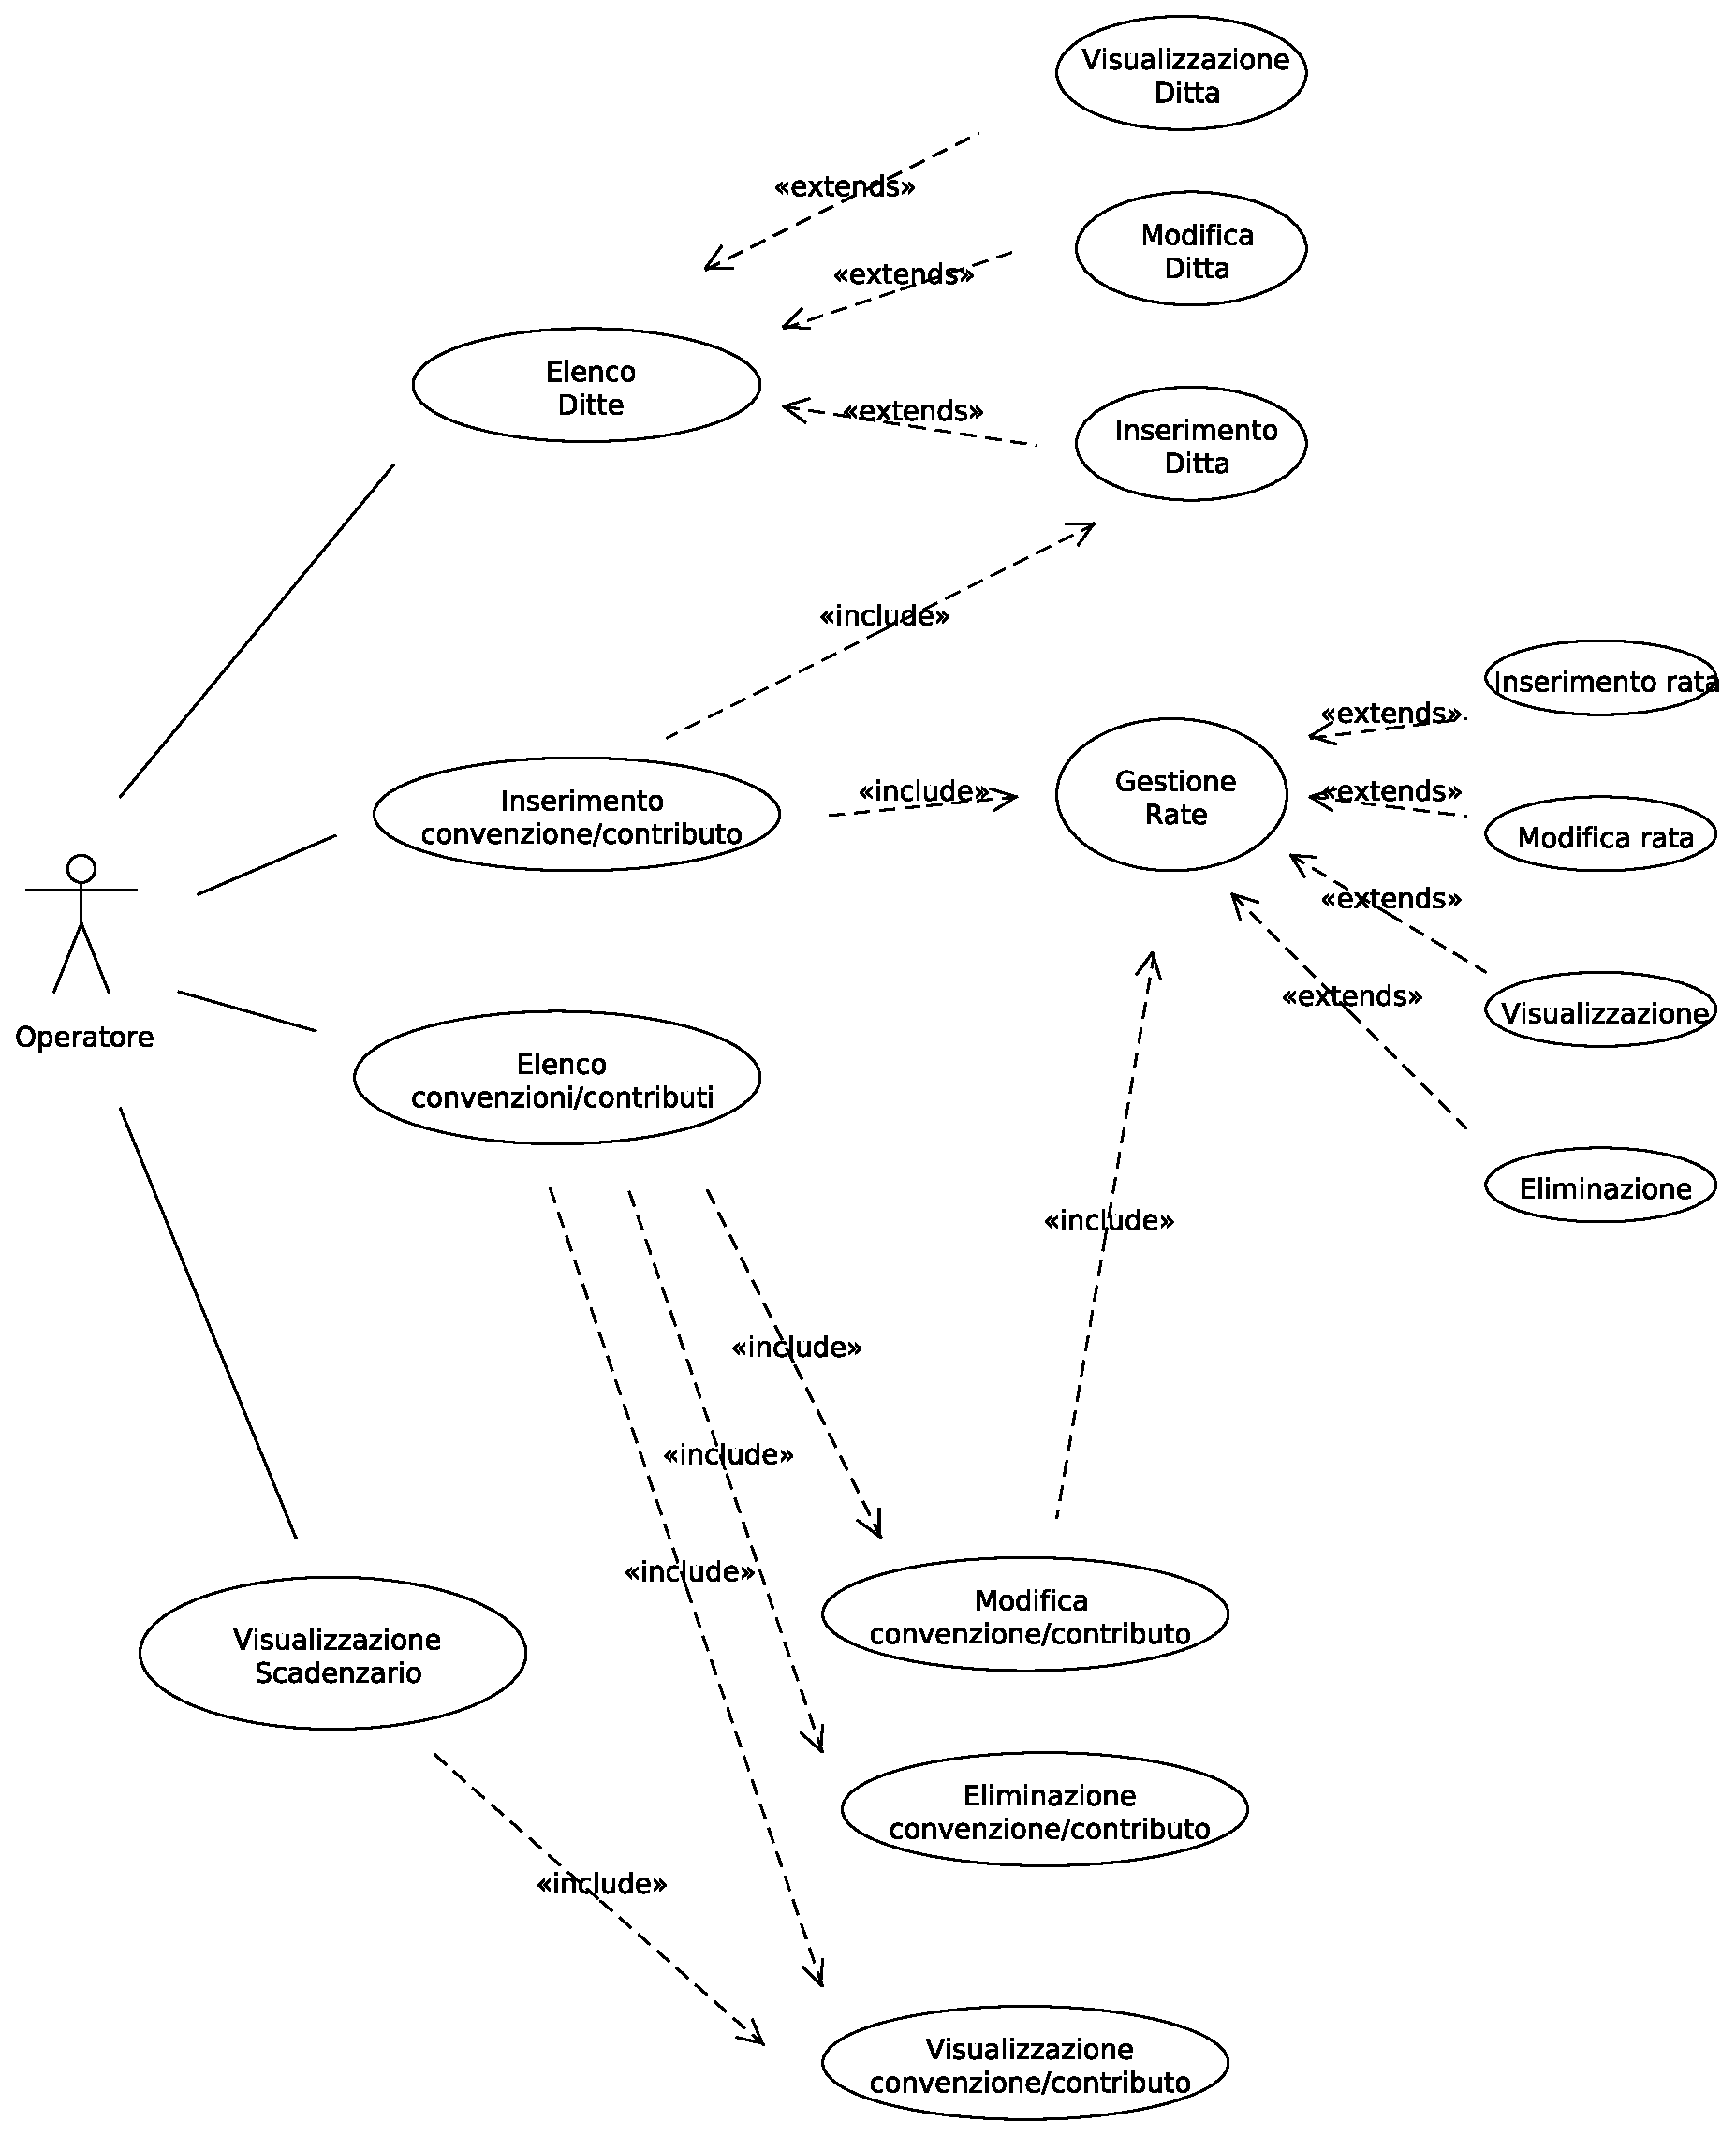
\includegraphics[height=0.8\textheight, width=0.7\textwidth]{images/casi_uso_operatore.eps}
    \end{figure}
  \end{frame}
  
  \begin{frame}{Casi d'uso del Docente}
    \begin{figure}[h]
      \label{use_case_diag_teacher}
      \centering
      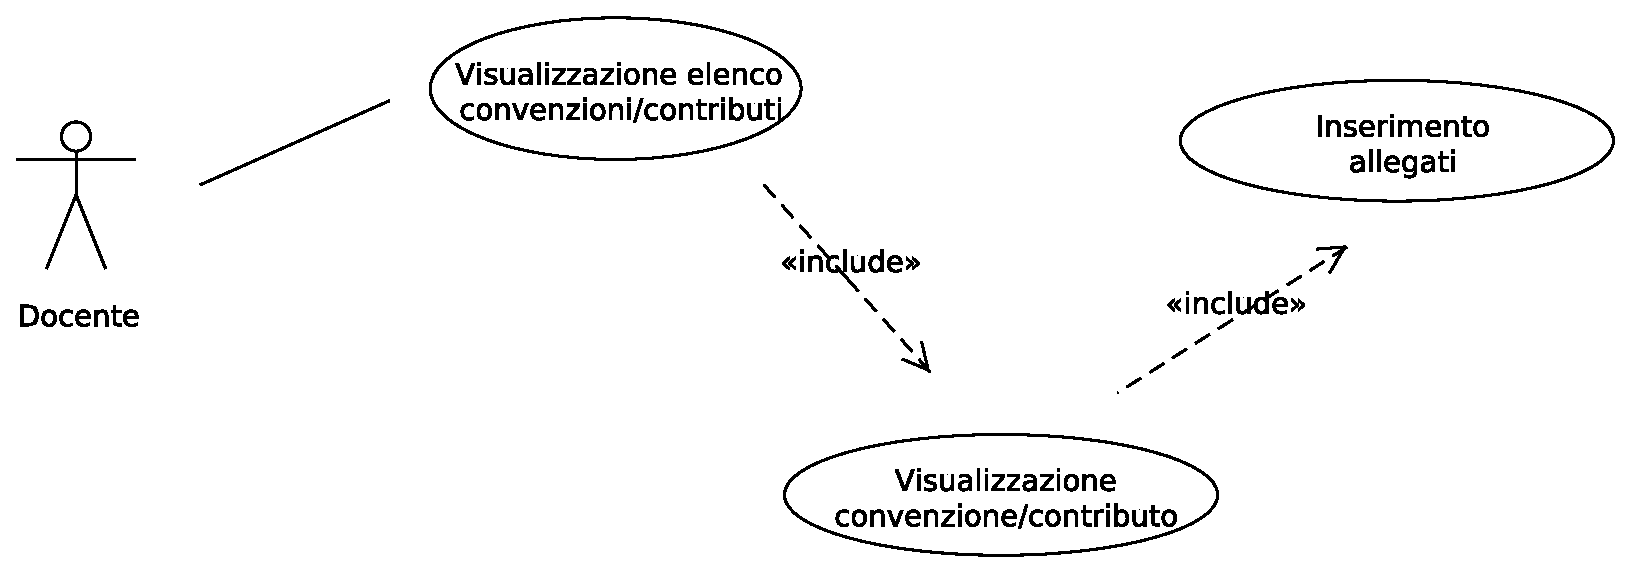
\includegraphics[width=0.8\textwidth]{images/casi_uso_docente.eps}
    \end{figure}
  \end{frame}
  
  \begin{frame}{Casi d'uso del Tempo}
    \begin{figure}[h]
      \label{use_case_diag_time}
      \centering
      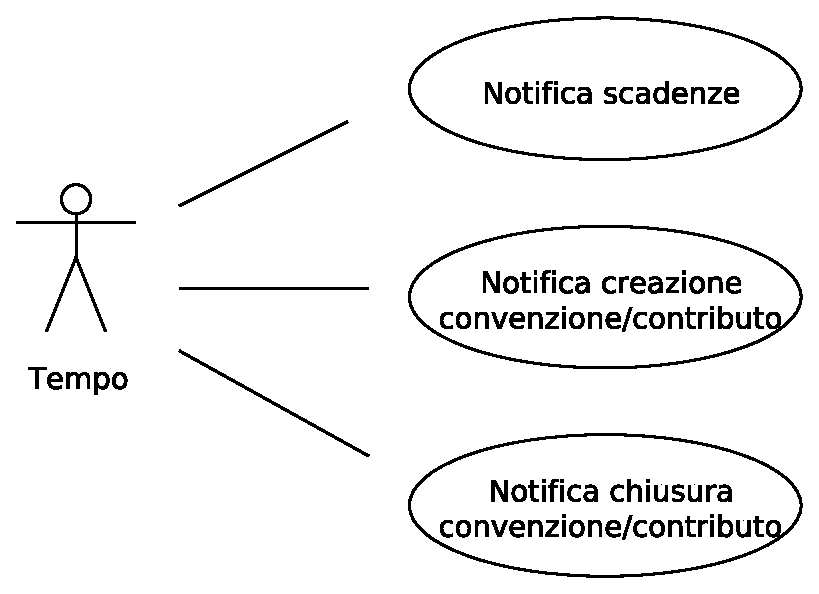
\includegraphics[width = 0.5\textwidth]{images/casi_uso_tempo.eps}
    \end{figure}
  \end{frame}


  
  \subsection{Modello di Business}



